\projecthead{02 / Flight \& propulsion}{3D-printed jet}{Airframe, propulsion \& flight-control development}{December 2025 - present}
\textit{In development}
\par\medskip A custom printed airframe with twin 80 mm electric ducted fans, developed around structural packaging, aerodynamics, and a target speed above 70 km/h.
\par\smallskip {\small\color{muted} Tools: Fusion 360, Inventor, Ansys Mechanical, Ansys Fluent, PyTorch}
\medskip
\noindent
\begin{minipage}[t]{.48\linewidth}\centering\vspace{0pt}
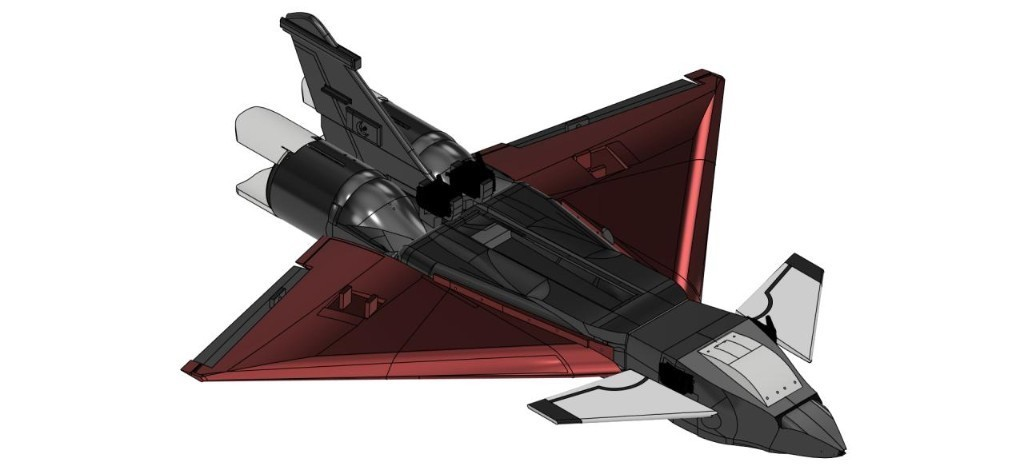
\includegraphics[width=\linewidth,height=1.8in,keepaspectratio]{images/jet/airframe.jpg}
\par\smallskip{\footnotesize\color{muted} CAD model of the airframe, fans, and tail.}\end{minipage}\hfill
\begin{minipage}[t]{.48\linewidth}\centering\vspace{0pt}
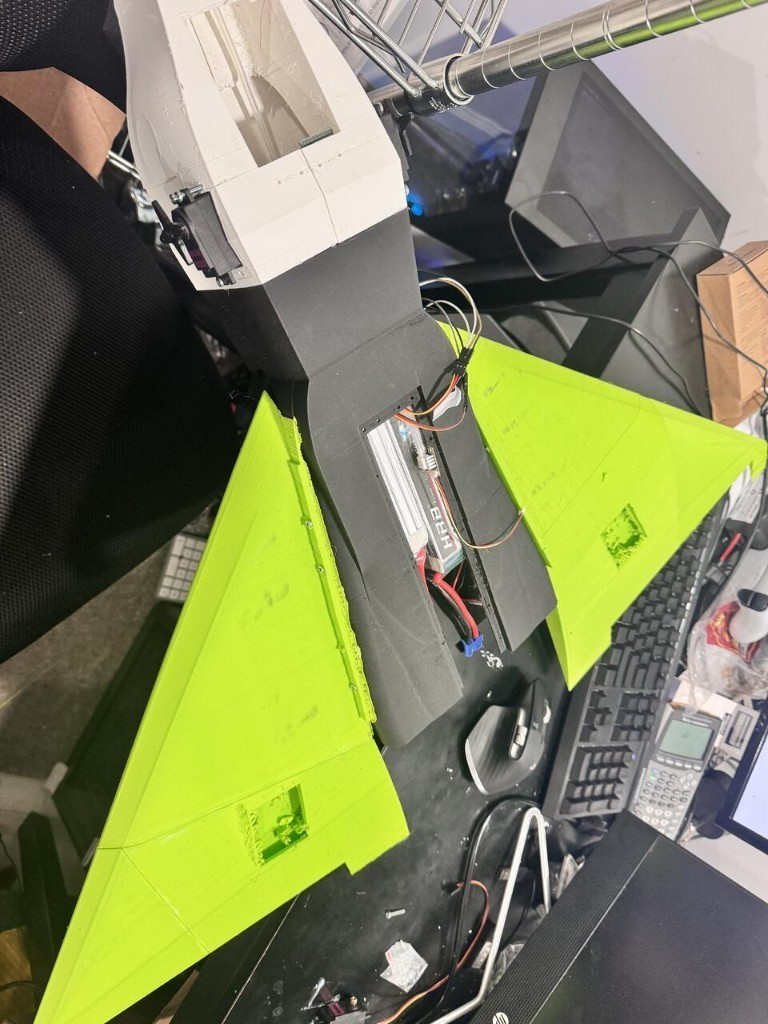
\includegraphics[width=\linewidth,height=1.8in,keepaspectratio]{images/jet/printed-wing.jpg}
\par\smallskip{\footnotesize\color{muted} Printed wing panels and battery bay.}\end{minipage}\hfill
\par\medskip
\noindent
\begin{minipage}[t]{.48\linewidth}\centering\vspace{0pt}
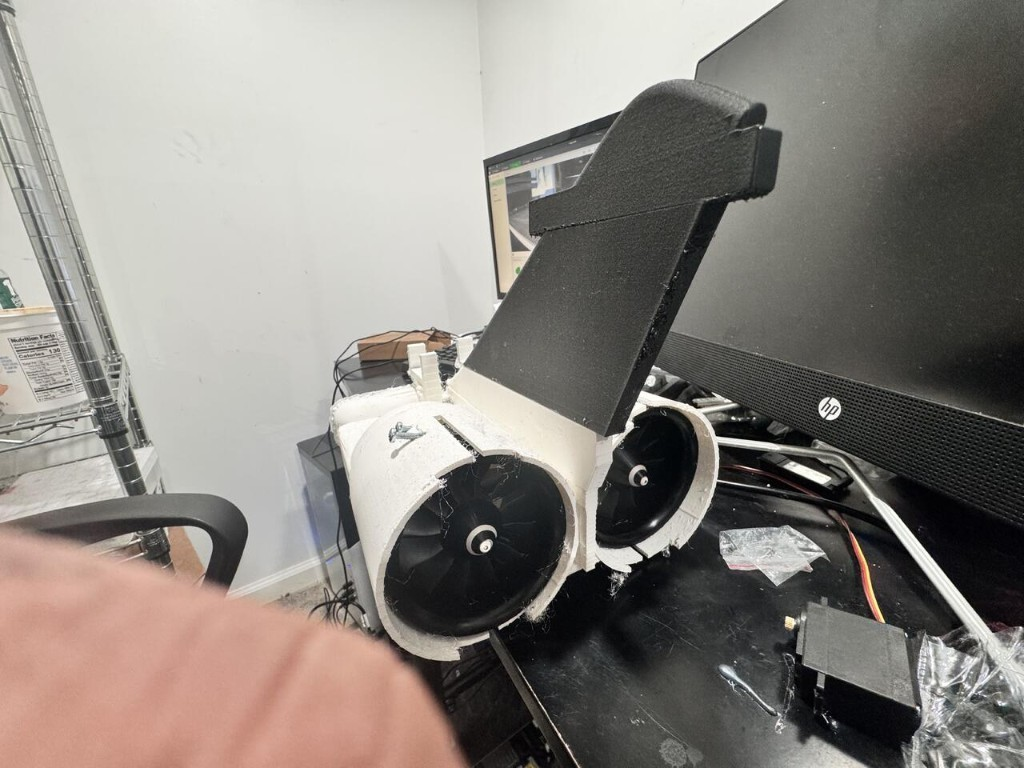
\includegraphics[width=\linewidth,height=1.8in,keepaspectratio]{images/jet/fan-assembly.jpg}
\par\smallskip{\footnotesize\color{muted} Twin fan ducts and tail during assembly.}\end{minipage}\hfill
\par\medskip
\subsection*{Airframe \& integration}
The airplane is drawn in Fusion 360 and printed in separate parts. The wing halves close over a battery bay, while two 80 mm electric ducted fans sit side by side at the rear.
\subsection*{Analysis \& control}
Structural and flow analysis inform the design. Thrust vectoring and onboard neural-network flight and landing control remain development goals. The 70 km/h figure is a design target, rather than a reported flight measurement.
\subsection*{Explore the model}
The original interactive aircraft model and flight demonstration remain available on the main website.
\medskip\href{https://muhammadmaalik.github.io/index.html?project=plane}{Explore the aircraft}